\section{Multi-Armed Bandit Problems}
\textbf{Setting:} A single state (aka situation) with multiple actions, one of which must be selected repeatedly. Each arm is slot machine with a stationary
probability distribution of rewards, say, $\mathcal{N}(\mu_i, \Sigma_i)$. The goal is to maximize the expected reward over some time horizon.

\begin{figure}[h]
    \centering
    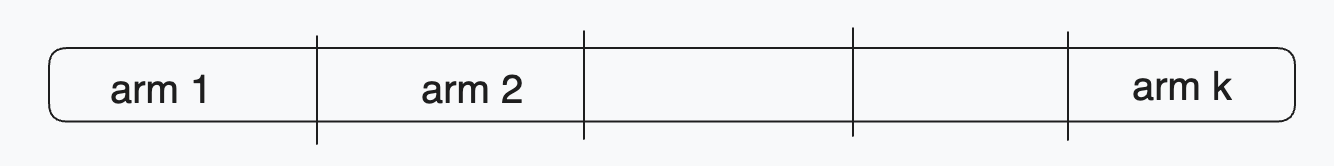
\includegraphics[width=0.9\textwidth]{img/bandit.png}
    \caption{A single state with multiple actions.}
    \label{fig:bandit}
\end{figure}


The expected reward of taking an action is given by:
\begin{equation}
    \begin{split}
        q_*(a) = \mathbb{E}[R_t | A_t = a] \\
        \label{eq:bandit}
    \end{split}
\end{equation}
This is the value of taking that action. We do not however know the value of each action, but we can estimate it by sampling the reward.
Thus, we approximate the value of an action as $Q_t(a) \approx q_*(a)$.

\subsection{Action-Value Methods}
Methods to estimate the value of an action and then use that estimate to select actions.

\subsubsection{Sample-Average Method:}
Each estimate is the average of all the sample of rewards collected up to that point.
\newline
Suppose $Q_t(a) = \frac{1}{N_t(a)} \sum_{i=1}^{N_t(a)} R_i$, where $N_t(a)$ is the number of times action $a$ has been selected up to time $t$.

\begin{equation}
    \begin{split}
        Q_t(a) = \frac{\sum_{i=1}^{t-1} R_i \cdot 1(A_i = a)}{\sum_{i=1}^{t-1} 1(A_i = a)} \\
        \label{eq:action-value}
    \end{split}
\end{equation}

\textbf{Action Selection:}
\begin{itemize}
    \item  Greedy: $ A_t = \text{argmax}_a Q_t(a) $
    \item  $\epsilon$-greedy: $ A_t = \begin{cases}
        \text{argmax}_a Q_t(a) & \text{with probability } 1 - \epsilon \\
        \text{random action} & \text{with probability } \epsilon
    \end{cases} $
\end{itemize}


With $\epsilon$-greedy, as $t \to \infty$, each action is sampled infinite times, and therefore the estimate $Q_t(a)$ converges to $q_*(a)$. 
The greedy selection, however, does not have strong convergence properties.

With `k' arms in  $\epsilon$-greedy method, the probability of selecting the greedy action is,
\begin{equation}
    \begin{split}
        P(\text{greedy action}) = (1 - \epsilon).P(\text{action is greedy}) + \epsilon.P(\text{action is random}) \\
        = (1 - \epsilon).1 + \epsilon.\frac{1}{k} \\
        = 1 - \epsilon + \frac{\epsilon}{k} \\
        \label{eq:epsilon-greedy}
    \end{split}
\end{equation}

The expected reward of the greedy action is TODO




